% !Mode:: "TeX:UTF-8"
% !TEX program  = xelatex
\documentclass[handout, aspectratio=1610, 14pt]{beamer}
\usepackage{amsmath, amssymb, bm, blindtext, braket, dsfont, extarrows, footmisc, graphicx, lipsum, siunitx, style, url, xcolor}

\usefonttheme{serif}
\usefonttheme{professionalfonts}

\addbibresource{ref.bib}

% %%%%%%%%%%%%%%%%%%%%%%%%%%%%%%%%%%%%%%%%%%%%%%%%%%%%%%%%%%%%%%%%%%%
% Some self-defined aliases. Feel free to delete or modify them.
\newcommand{\operator}[1]{\hat{\bm{#1}}}
\newcommand{\hl}[2]{\colorbox{#1}{#2}}
\newcommand{\OD}{\text{OD}}
\newcommand{\itmspace}{\vspace{5pt}}
\renewcommand{\Im}[1]{\operatorname{Im}{\{#1\}}}
\renewcommand{\Re}[1]{\operatorname{Re}{\{#1\}}}
% %%%%%%%%%%%%%%%%%%%%%%%%%%%%%%%%%%%%%%%%%%%%%%%%%%%%%%%%%%%%%%%%%%%

\begin{document}
\title{Your Defense Title}
\author{\texorpdfstring{Your~Name\\{\scriptsize \url{name@connect.ust.hk}}}{Your~Name}}
\supervisor{Prof.~Your~Supervisor}
\institute{Department of Physics, HKUST}
\date{2020/11/30}

% Title Page
\frame{\titlepage}

% TOC Page
\begin{frame}
\frametitle{Contents}
\makecontents
\end{frame}

% Section: Introduction
\section{Introduction}

\begin{frame}{Introduction}
  \begin{figure}[!h]
    \centering
    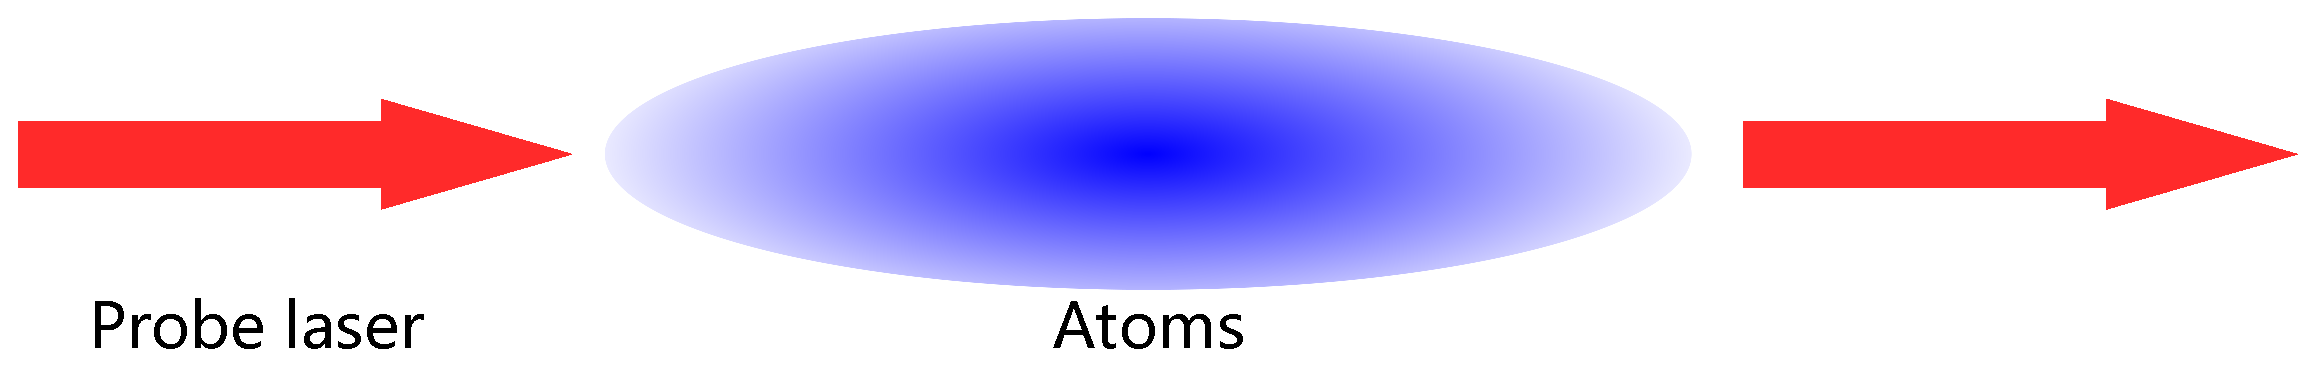
\includegraphics[width=0.9\textwidth]{figure/Atoms.eps}
  \end{figure}

  \begin{itemize}
    \itmspace
    \item EIT and slowlight in Rubidium 85 atom system\itmspace
    \item Dephasing affects the efficiency\itmspace
    \item Control the magnetic filed to decrease dephasing
  \end{itemize}
\end{frame}

% Section: Theory
\section{Theory of light-atom interaction}

\subsection{EIT and Slowlight in Three-level system}

\begin{frame}{Three-level system}
  \begin{equation*}
    \hat{H}_{\text{eff}} = \hbar 
    \begin{matrix}
      \begin{pmatrix}
        0 & 0 & -\frac{1}{2}\Omega_p^{*} \\
        0 & -\delta - \frac{i\Gamma_2}{2} & -\frac{1}{2}\Omega_c^{*} \\
        -\frac{1}{2}\Omega_p & -\frac{1}{2}\Omega_c & -(\Delta+\delta) - \frac{i\Gamma_3}{2}
      \end{pmatrix}
    \end{matrix}
  \end{equation*}
  
  coupling detuning: $\Delta = \omega_c - (\omega_3 - \omega_2)$
  
  probe detuning: $\delta = \omega_p - \omega_c - (\omega_2 - \omega_1)$
  
  \begin{equation*}
    a_3 = \frac{2\Omega_p (\delta+\frac{i\Gamma_2}{2})}{|\Omega_c|^2 - 4(\Delta+\delta+\frac{i\Gamma_3}{2})(\delta+\frac{i\Gamma_2}{2})}
  \end{equation*}
  \begin{equation*}
    \chi = \chi(\delta) = \frac{N|\mu_{13}|^2}{\epsilon_0 \hbar} \frac{4(\delta+i\textcolor{red}{\frac{\Gamma_2}{2}})}{|\Omega_c|^2 - 4(\delta+\Delta+i\frac{\Gamma_3}{2}) (\delta + i\textcolor{red}{\frac{\Gamma_2}{2}})}
  \end{equation*}
\end{frame}



% Section: System
\section{System Configuration}

\subsection{MOT and Optical layout}

\begin{frame}{MOT and Optical layout}
  \begin{columns}[onlytextwidth]
    \hspace{10pt}
    \begin{column}{0.6\textwidth}
      \includegraphics[width=\textwidth]{example-image}
      \vspace{-30pt}
      \begin{center}
        Circuit (see appendix)
      \end{center}
    \end{column}
    \hspace{-30pt}
    \begin{column}{0.5\textwidth}
      \begin{minipage}{\textwidth}
        \vspace{-5pt}
        \begin{figure}[!h]
        \centering
        \includegraphics[width=0.6\textwidth]{example-image}
        \end{figure}
        \vspace{-25pt}
        \begin{center}
          Hall probe
        \end{center}
      \end{minipage}
      \begin{minipage}{\textwidth}
        \begin{figure}[!h]
        \centering
        \includegraphics[width=0.6\textwidth]{example-image}
        \end{figure}
        \vspace{-25pt}
        \begin{center}
          Bias coil design
        \end{center}
      \end{minipage}
    \end{column}
  \end{columns}
\end{frame}


% Section: Experiment
\section{Experiment}

\subsection{Adjust switch-off device and bias coil}

\begin{frame}{Adjust switch-off device}
\blindtext
\end{frame}


% Section: Conclusion
\section{Conclusion \& Outlook}

\begin{frame}{Conclusion \& Outlook}
\begin{itemize}
    \item Conclusion\vspace{5pt}
    \begin{itemize}
        \item \lipsum[66]
    \end{itemize}
    \vspace{10pt}
    \item Outlook\vspace{5pt}
    \begin{itemize}
        \item Automatically adjust the bias currents by computers and tools like machine learning\cite{machineLearning}\vspace{4pt}
    \end{itemize}
\end{itemize}
\end{frame}

% Section: Appendix
\section*{Appendix}

\begin{frame}{Appendix: ...}
The circuit for the project is:
\begin{figure}[!h]
    \centering
    \includegraphics[width=0.6\textwidth, height=0.6\textheight]{example-image}
\end{figure}
\end{frame}


% Ending Page
\begin{frame}
\thanks
\end{frame}

\end{document}
